\subsection{The state of the art in theoretical frameworks for dark matter}
\label{sub:stateOfTheArtTheory}
\smallskip
%CD: The idea is not to have two separate DM and theoretical framework sections, but rather have everything in ~1 page with much sharper concepts (AB comment "misses the point" had a point).  

%Aims of this paragraph: DM and why should we look for it at the LHC
Gravitational and cosmological observations~\cite{Bertone:2016nfn} point to the existence of dark matter, for which the SM does not provide any explanation. 
Many mechanisms explaining the present amount of dark matter in our universe (called \textit{relic density}) imply that, if DM is a new particle, it must have a connection with SM particles~\cite{Hall:2009bx,Bernal:2017kxu,Steigman:2012nb}~\footnote{Alternative mechanisms and explanation for DM exist, e.g.~\cite{McGaugh_2016,Lennon:2017tqq,Bird:2016dcv,Marsh:2015xka}. Given our ignorance on the genesis of DM, pursuing a broad theoretical and experimental approach that considers different possibilities is motivated and advocated in WP5.}. 
%[CD: am I digging myself a hole? Also using the word genesis is not ideal. Also is a fun read: http://inspirehep.net/record/1711655] 

%Aims of this paragraph: introduce the WIMP and complementarity between ID/DD/LHC
A popular DM candidate satisfying the relic density is the WIMP, a TeV-scale stable particle with interaction strength comparable to the weak force.  
Owing to these characteristics, WIMPs are detectable by a variety of experiments. 
Indirect detection experiments (ID) could observe excesses of SM particles over astrophysical backgrounds due to WIMP annihilation in DM-rich regions. 
Direct detection experiments (DD) could detect the interaction between incoming WIMPs and recoiling target nuclei within the detector. 
The LHC could produce DM from collisions of SM particles in controlled conditions, allowing for an exploration of DM-SM interactions. 
A LHC discovery, matched to a DD and ID discovery~\footnote{Particles that look like DM in LHC experiments may decay after leaving the detector, with a lifetime incompatible with DM’s cosmological timescales.}, can shed light on the particle nature of WIMP dark matter. 
\\
\indent 
Exploiting \textbf{synergies between different experiments} in terms of common discovery potential requires a well-specified \textbf{common theoretical ground}. 
%Aims of this paragraph: introduce simplified models, introduce Z' and its parameters, justify their use (too many aims?)
WIMP DM models range from fully-specified theories such as supersymmetry (SUSY)~\cite{Martin:1997ns} to effective field theories (EFT) at energy scales where the exact details of the interaction can be ignored~\cite{Goodman:2010ku}. 
During the course of my StG, I co-led the Dark Matter Working Group and produced a series of recommendations that would define the state-of-the-art for benchmark models for generic LHC DM searches~\cite{Abercrombie:2015wmb}. 
These focused the community around \textbf{simplified models} that reproduce relevant experimental features using a limited number of parameters. 
Simplified models introduce a new particle acting as the mediator of the interaction between ordinary matter and dark sector particles, as a step forward from EFTs. 
This mediator can be a spin-1 particle analogous to the Z boson (a $Z’$ boson)~\cite{Shoemaker:2011vi,Buchmueller:2013dya,Chala:2015ama}, a new spin-0 scalar much like a new Higgs boson~\cite{Buckley:2014fba,Egana-Ugrinovic:2019dqu,Abe:2018bpo}, or a spin-2 graviton~\cite{Kang:2020huh}. 
%Here I want to show completeness
Models including a vector and scalar mediator have been used to benchmark the sensitivity of future facilities and compare it to the next-generation DD and ID experiments, as input to the update of the European Strategy of Particle Physics~\cite{Strategy:2019vxc}.
This complementarity of DD, ID and LHC experiments~\cite{Bauer:2013ihz} is fully rooted in the LHC DM search program and has been established during the course of my StG~\cite{Boveia:2016mrp}.
\indent
While additional interactions and modifications are required to make simplified models self-consistent (see e.g.~\cite{Ellis:2018xal}), they do not change the main experimental feature: given that the mediator has been produced from the interaction of SM particles, then it can also decay into SM particles. 
Sensitivity to these visible mediator decays gives LHC experiments unique insight into the dark sector. 
An astrophysics discovery of DM could be further characterized in terms of the interactions between the mediator and its SM decay products, 
and a LHC discovery of a mediator particle supported by relic density measurements could focus attention at particular regions in DM parameter space. 

\begin{wrapfigure}{R}{0.65\textwidth} 
\begin{center}
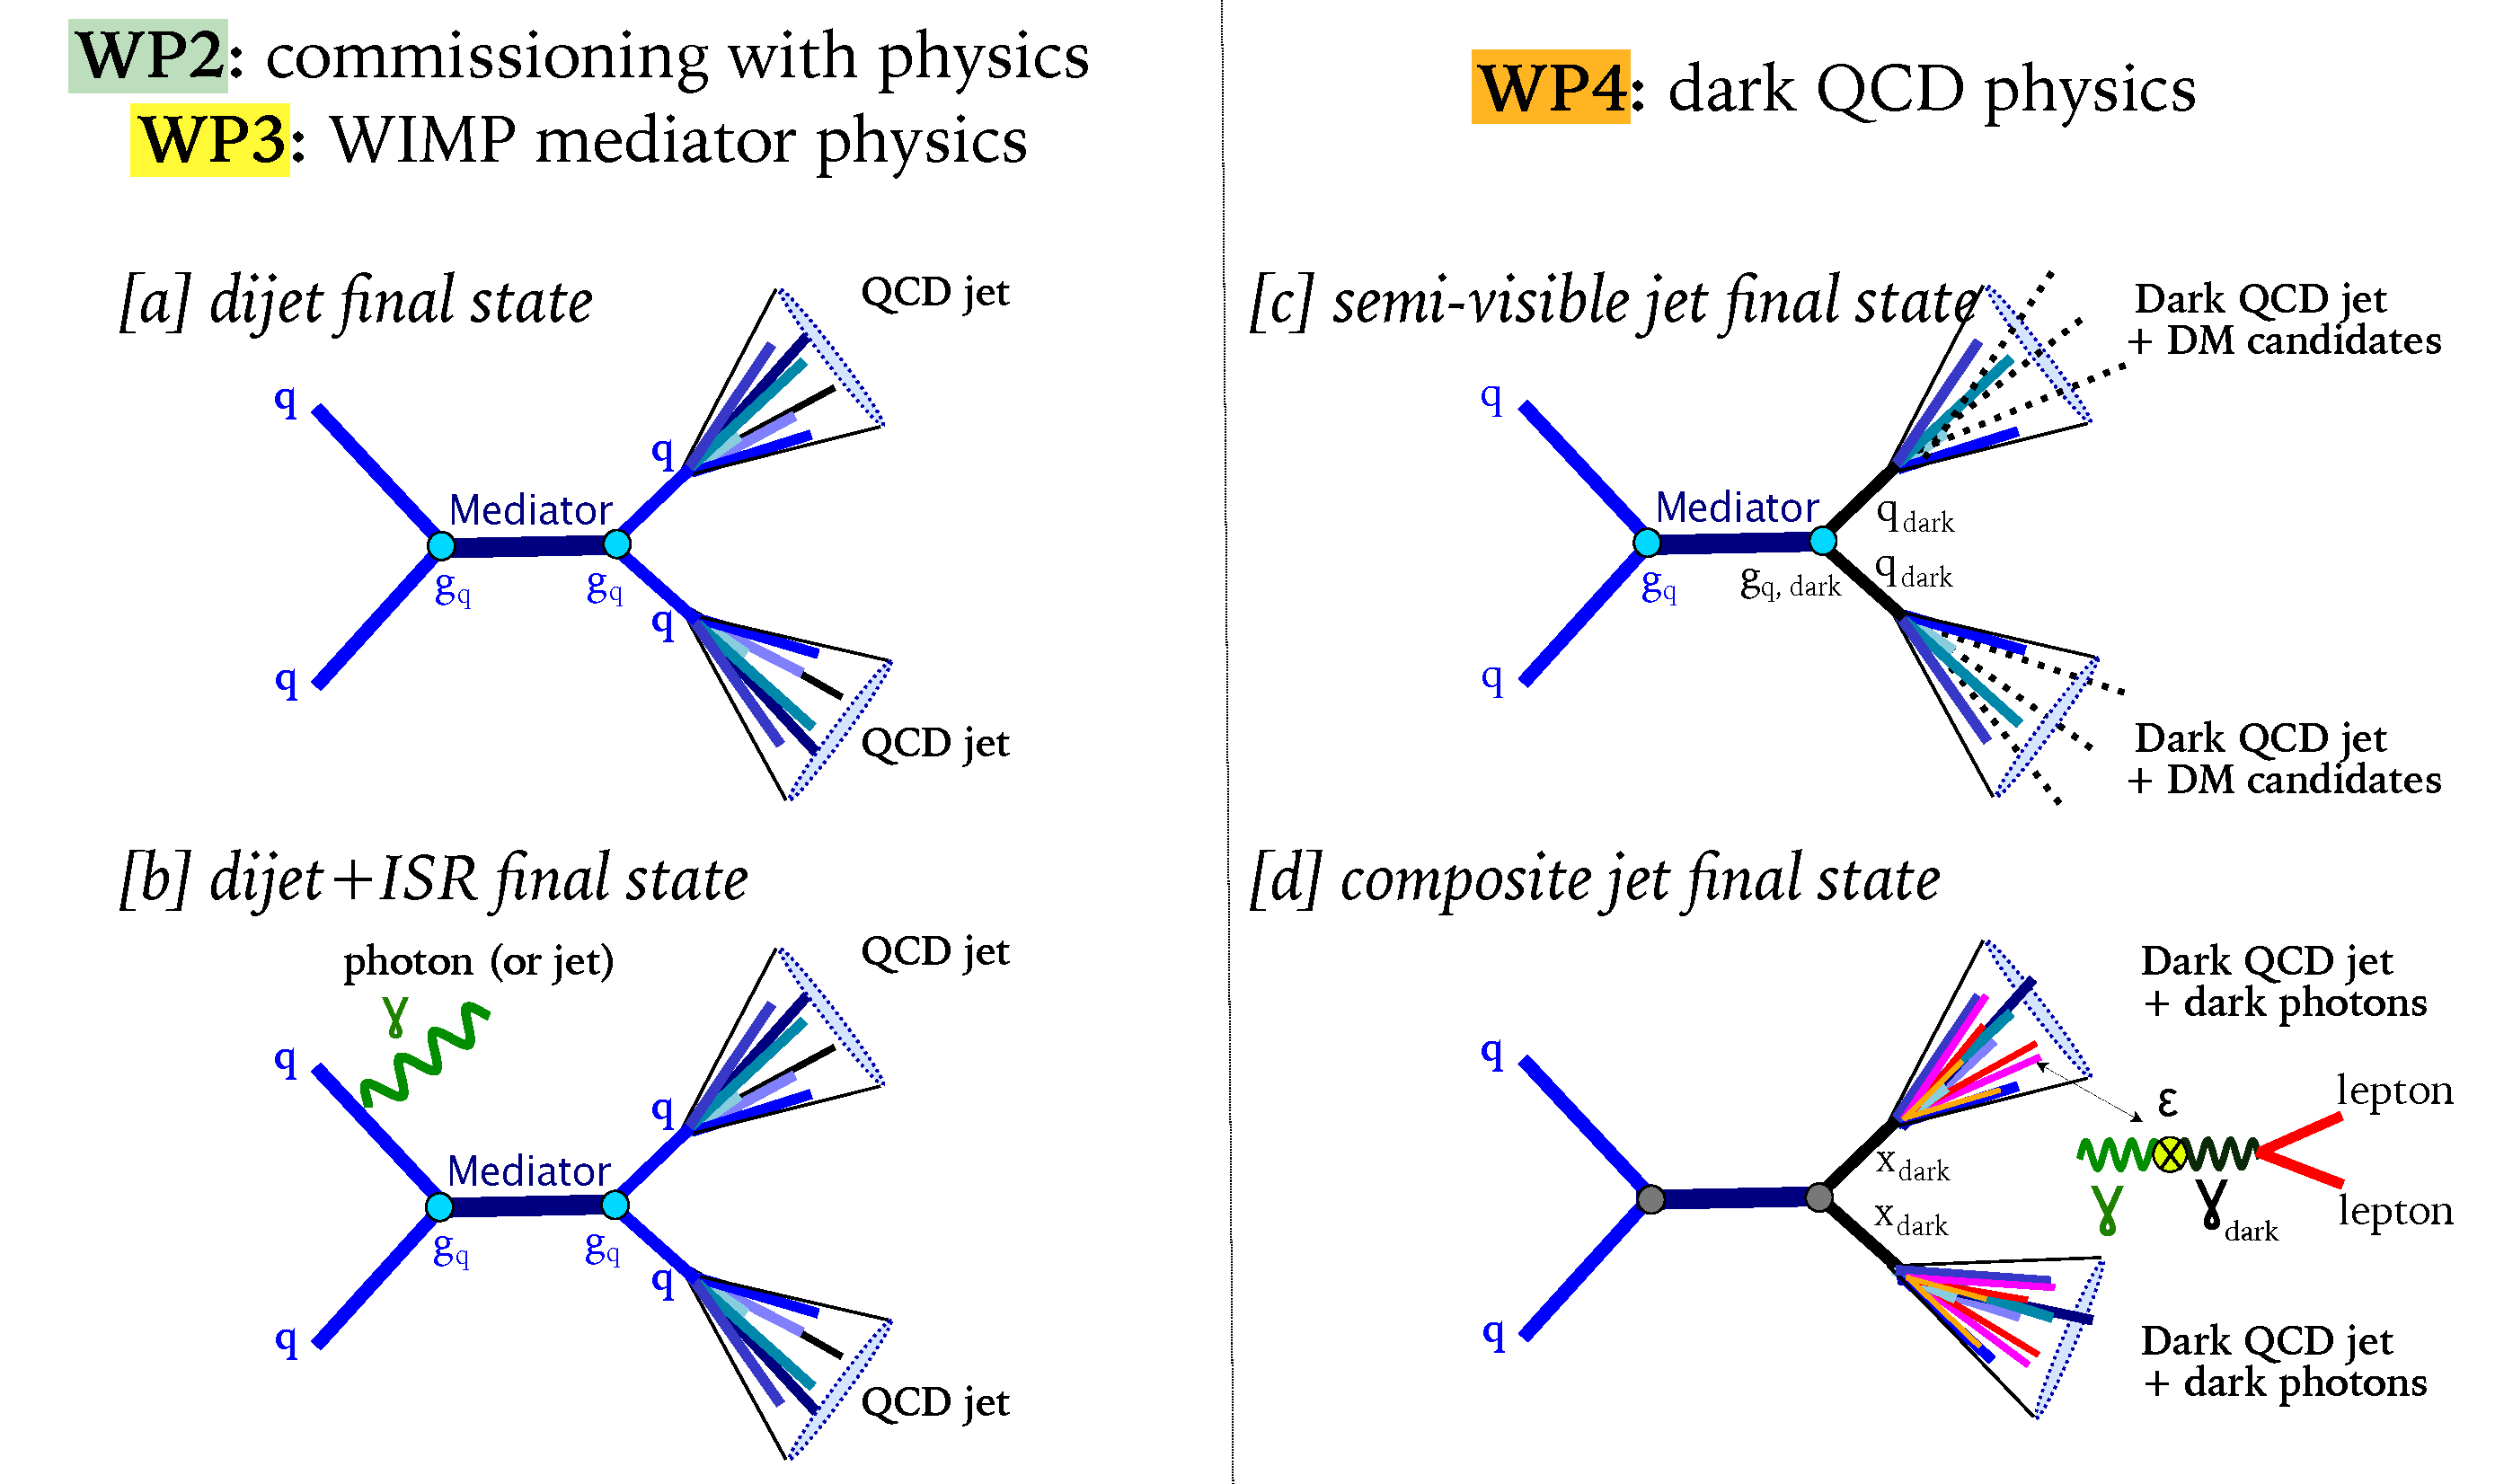
\includegraphics[width=0.65\textwidth]{figs_B2/feynman.pdf}
\caption{Sketches of search signatures in this proposal.\color{black}\label{fig:feynman} }
\vskip2pt
\end{center}
\end{wrapfigure}
%\vskip5pt

Simplified models are well-motivated benchmarks at a time when no experimental hints are observed, as they allow for a systematic exploration of experimental search targets by scanning the parameter space (DM mass $m_{DM}$, mediator spin and mass $m_{Med}$, couplings to DM $g_{DM}$ and SM $g_{SM}$).
Exploration of yet unprobed parameter space for mediator decays as in the left-hand side of Fig.~\ref{fig:feynman} motivates the searches in WP2 and WP3. 

%More to defend simplified models, maybe too much?
%Furthermore, motivating searches for only a handful of new particles with simple interactions even if they are part of a complex spectrum is conceptually supported by how ordinary particles were uncovered in the history of the SM: the first particles discovered were the most common ones, and further complexity was unraveled at a later date. 
%These searches will be used to commission trigger improvements in WP2-3 will improve  much greater sensitivity with respect to previous searches , and employ simplified models as building blocks for more complex theories (WP4). 

%Aims of this paragraph: introduce dark sector models and hidden sector
In parallel to considering WIMP DM models, it is also imperative to \textbf{consider alternative DM models that could have escaped detection} so far. 
An example is a class of models including mediator-like particles that do not directly connect DM and SM, but rather provide a \textbf{hidden portal} with much weaker interactions between a more complex dark sector and SM particles~\cite{Strassler:2006im}. 
\\
\indent
The symmetries of the SM can be used as guiding principle to construct the particle spectrum and the interactions of the new dark sector. 
A \textbf{new $U(1)$ symmetry} introduces a portal particle called \textit{dark photon}~\cite{Holdom:1985ag,Curtin:2014cca}.   
The dark photon mixes with the ordinary photon, leading to rare but observable signatures from its decays to SM particles. 
This model is currently used as a benchmark for many non-LHC experiments and for future facilities~\cite{Strategy:2019vxc}. 
%Why according to Shaposhnikov (who motivated benchmarks): doesn't quite convince me. 
%Light particles have become a more popular search target because they can be used to solve particle physics  
%g-2, only in connection with DM
%and astrophysics anomalies 
%Pamela (bleurgh)
%too-big-to-fail as opposed to WIMPs - self-interactions
Models with a \textbf{new SU(2)}, also termed \textit{dark QCD} models for their similarity with SM QCD, predict that their fundamental components (dark quarks, $q_{dark}$) are confined at an energy scale that can be comparable to that of QCD. 
This leads to signatures of highly collimated particles, resembling hadronic jets that include dark sector particles and their decay products (\textit{dark jets}). 
\\
\indent
A number of concrete realizations of theories including one or more of those new symmetries exist (e.g. asymmetric DM~\cite{Zurek:2013wia}, electroweak SUSY models~\cite{Cheung:2009su}, self-interacting DM~\cite{Tulin:2017ara}, strongly-interacting DM~\cite{Bernreuther:2019pfb}). 
The large number of parameters and particles, and their subsequent variability in terms of experimental manifestations, mandates \textbf{signature-driven searches} rather than searches targeting specific theory benchmarks. 
For this reason, the data-taking techniques in this proposal are designed to \textbf{record data that could contain a variety of these signatures, and that would otherwise be discarded}. The searches in WP4, using the dark jets signatures shown in the right-hand side of Fig.~\ref{fig:feynman} \textbf{target two uncovered dark sector signatures} as concrete use cases for this dataset. As shown in the right-hand side of Fig.~\ref{fig:feynman}, we will first search for dark jets containing thermal relic DM particles (semi-visible jets) produced from the decay of a $Z’$~\cite{Bernreuther:2019pfb,Cohen:2017pzm}, and subsequently for dark jets where the showering process interleaves dark photons and dark hadrons, leading to hadronic jets with an anomalous leptonic content (composite jets)~\cite{Cheung:2009su,Park:2017rfb}.
%Further thoughts are in here
%%Together or individually, mediator particles above and dark photons can also be part of a dark sector set of particles that do not interact significantly with the SM, including the DM candidate~\cite{Felix}. 

%Another possible story (but longer)
%Building blocks: dark QED
%Why attractive
%Conceptual connection to vector mediator above
%Why neglected
%Next-on: dark QCD
%Why attractive
%Why neglected




%For this reason, systematic exploration of these models does not proceed by scanning the theory’s parameter space, but rather by mapping the characteristics of different possible configurations of parameters and ensuring that no experimental stone is left unturned. 
%Searches for this kind of models have recently started taking shape at the LHC, in parallel to a vigorous pursuit by planned and existing non-LHC experiments~\cite{PBC}. 



%DM can't catch light DM even though there are a lot of tries
%So we go after the mediators again

%- Large experimental variability
%- Many motivations for lepton-jet models, but they neglect hadronic dark sector particles (eg SUSY lepton-jets below)
%- So we start where we can, and where we have motivations - B-L? 

%Peter's suggestion for B1, but I don't know where to add it? 
%The only thing I miss and I can understand that it can be hard to fit in is a motivation of WIMPs and
%in particular dark QCD. Could one maybe add just a little a la:
%The nature of dark matter is difficult to understand, because even today there is five times more
%dark matter than normal matter, this is only after essentially all normal matter in the Universe
%annihilated microseconds after the Big Bang (only 1 in 10,000,000,000 protons survived). The WIMP
%solution is a weakly coupled particle that yields the observed DM abundances by being weakly
%produced. It is attractive to search for WIMPs at the LHC because the energy of the accelerator
%allows studies above and below the electroweak phase transition. In Dark QCD one instead assumes that
%the abundances are similar because there also was an annihilation in the dark sector of the Universe
%and so Dark QCD models can potentially also explain the matter-antimatter symmetry observed in the
%Universe. It is attractive to search for Dark QCD at the LHC because it is a QCD collider and so one
%could expect that if there is a coupling between QCD and Dark QCD then we are likely to produce Dark
%QCD mesons and baryons at the LHC.%Check the latter

%SUSY lepton-jets: https://arxiv.org/pdf/0909.0290.pdf
%The cascades to N ̃1 may also result in colored particles and hence QCD-jets, but for the purpose of the current study we will assume that a substantial fraction of such cascades result in no colored particles. This is not a strong assumption as it is satisfied in many concrete examples of MSSM spectra [11], and may even be discarded altogether in actual lepton jet searches including QCD-jets.

%Existing text
%, and as a consequence it is only extremely feebly connected to electrically charged particles - I should probably talk about its decays
%too ambiguous? it decays into fermions as if it were a photon
%rather than direct interactions with


%This is one of the cases in which simplified models are used as building blocks for more complex models.


%In WP4, I will make use of my expertise in the reconstruction of hadronic jets and non-standard data taking technique to search for two classes of theoretically-motivated DM models that include a new strong force within the dark sector (dark QCD), using novel data taking techniques necessary for uncovering their signatures. 
%With these searches, this proposal will contribute to the systematic mapping of the territory of hidden sector signature, in synergy with other LHC and non-LHC searches. 

The emergence of new models for DM and new ways to look for them indicates that the DM community is thriving.  
Depending on the SM-DM interaction strength and on the DM characteristics, a wealth of new experiments can contribute to the quest for WIMP and non-WIMP DM~\cite{Beacham:2019nyx,Bertone:2019irm,Barausse:2020rsu}. 
It is clear that, given the breadth of possible explanations for DM, an equally broad experimental and theoretical approach is needed, 
and that new synergies can be exploited beyond the already-mentioned complementarity between DD/ID and colliders searches. 
This consideration inspires the work planned for WP5, taking place within newly established common platforms for dissemination of results and tools, in the spirit of open and collaborative science. 

\subsection{The state of the art in experimental tools for discovering dark matter and new phenomena}
\label{sub:stateOfTheArtExperiment}

\subsubsection{LHC and ATLAS: overview and schedule}
\smallskip

The LHC will restart operations in Summer 2021 and continue delivering proton-proton collision data until the end of 2024. In this data taking period (called \textit{Run-3}), up to 250/fb will delivered to the ATLAS experiment~\cite{ATLAS2008}.%{JINST2008}. 
It is expected that the bulk of the data will be collected in 2022 onwards, after a first period of commissioning for the machine and the experiments. 

In Run-3, the LHC collision energy will not be significantly increased, and the dataset size will be only slightly larger than the Run-2 dataset (189/fb). 
It is clear that the discovery potential warranted by the upcoming dataset will not improve by statistics alone. 
\textbf{New methods and technical innovations are required to discover rare processes}, at a time when traditional data-taking confirms the SM.%, mandates technical innovation. 
Innovating the ATLAS data acquisition and selection system is an integral part of this proposal, 
as the key to extract a much larger amount of useful information from the upcoming LHC dataset. 
This proposal is especially timely given that the improvements within \textsc{Realdark} can be tested with physics in early data and are required to be made in advance of the LHC production phase for full exploitation of the LHC dataset. 

\subsubsection{The ATLAS trigger and its upgrades}
\smallskip

Recording the entirety of the LHC data (up to 30 million collision events/second) is unfeasible due to storage and computing limitations. 
Therefore, \textbf{only a small fraction of interesting events is selected} by the ATLAS trigger system. 
%The rest are discarded forever. 

The ATLAS trigger is composed of two levels~\cite{ToBeCited}. %2015TriggerPaper
The first hardware level (L1) performs an initial coarse selection within 2.5 $\mu s$. 
Selected events are passed to the software-based High Level Trigger (HLT), implemented on a computing farm. 
The HLT performs a more refined event reconstruction and data analysis \textit{online}. 
This informs the final decision on whether to discard the event or keep the full detector information for further \textit{offline} reconstruction and analysis of electrons, muons, photons, jets, ... (called \textit{physics objects} in the following). 
The total event rate that can be retained after the HLT decision is directly \textbf{limited by the available amount of storage space}. 
%since traditional offline analysis currently requires the full set of detector information for reconstruction of physics objects (e.g. electrons, muons, photons, jets...). 
The rates of useful events recorded for offline analysis are also indirectly limited by the available HLT computing: 
a number of high-level features that would help in distinguishing signal from background are \textbf{too expensive to reconstruct given the available HLT resources}. 
%An example of such a feature is the track-collision vertex association for physics objects, 
%as this enables removing spurious contributions from simultaneous proton-proton collisions other the one of interest (pile-up). 
These limitations impairs the sensitivity of searches where signals are buried in high-rate backgrounds and motivates the improvements in WP1. 

The ATLAS trigger is undergoing significant upgrades for Run-3~\cite{Aad:1602235}. 
The ATLAS L1 trigger will be equipped with new electronic boards that allow for a more granular and efficient first-pass selection. 
As part of my StG, my team has developed control software for the board which will permit using information from the entire hadronic calorimeter at once (gFEX)~\cite{Tang:2016ded}, 
and contributed to the software for the new jet board (jFEX)~\cite{Bauss:2018nde}. 
The computing power of the ATLAS HLT farm will increase significantly, and optimized trigger tracking algorithms will be available~\footnote{See 
Ref.~\cite{ATL-PHYS-PUB-2019-041} %Elsing 
for an example of the improvements from optimizing tracking algorithms on simulated data containing 200 simultaneous collisions for the ATLAS high luminosity upgrade}. 
This will enable a more widespread availability of tracking at the trigger level, allowing to reject backgrounds from simultaneous proton-proton interactions (pile-up). Testing and exploiting these upgrades is an integral part of this proposal. 

%Among those, a full overhaul of the electronic boards that read in calorimeter information is foreseen. 
%The board that reads information from the electromagnetic calorimeters (eFEX) will allow for more refined distinction between electrons and photons already at L1. 
%This motivates the implementation of alternative data-taking techniques to overcome these limitations, as proposed in WP1 and discussed in the next section. 
%This can probably be removed since I don't use it directly anywhere else? 

\subsubsection{Review of analysis strategies for DM and related particles at the LHC}

Traditional searches for \textbf{WIMP Dark Matter} at colliders seek an excesses of imbalanced events where weakly or non-interacting particles escape the detector unseen~\cite{Boveia:2018yeb}. 
If the processes sought in traditional searches via a mediator particle as described in Ref.~\ref{sub:stateOfTheArtTheory}, 
resonant signals should also be present from the decays of the mediator into SM particles.
Searches for visible decays of the mediators are complementary to searches for invisible particles~\cite{CMSSummary,ATLASSummary}  
%Another point to look for visible decays, but not relevant here: 
%Considering the simple picture of \textbf{Fig. X}, invisible signals will be suppressed with respect to visible signals if the DM particle is much heavier than the particle mediating the interaction and invisible decays must occur off-shell. 
%\textbf{Decide: dijet/di-jet}
%Searches for visible signatures is an established complementary alternative to searches for invisible particles, with different challenges and sensitivity~\cite{ToBeCited}.%Summary plots 
Visible mediator decays connect DM mediator searches with the well-known class of searches for new resonances at particle colliders. 
New resonant particles have a large array of theoretical motivations beyond DM, and are not yet fully constrained by existing searches~\cite{Kim:2019rhy}%{Craig2bodyResonances} 
\\
\indent
The searches in WP2 and WP3 in this proposal focus on a well-motivated yet experimentally challenging category of decays (see e.g.~\cite{Chala:2015ama}). 
Having been produced via a quark-quark vertex, the mediator will also decay back into quarks (Fig.~\ref{fig:feynman} [a]). 
The signature of this process is a resonant peak in the two-jet (dijet) invariant mass, peaking atop the smooth QCD background.
%%The relatively low background rates of high-mass hadronically-decaying resonances permit collecting all events in full above a threshold of approximately 1 TeV~\cite{ToBeCited}. 
Below 1 TeV, large amounts of QCD backgrounds overwhelm the experiment’s data storage resources, forcing to discard signal together with background~\cite{ToBeCited}. %high-mass dijets  
For this reason, dijet resonances with masses around the electroweak scale ($\approx$100-200 GeV) have been very difficult to probe with standard data-taking techniques. 
\\
\indent
Discovering \textbf{resonances with sub-TeV masses require novel data taking techniques and/or targeted signatures}. 
%During my StG, my team and I have pursued both directions within ATLAS. 
Following the example of the Data Scouting technique in CMS~\cite{ToBeCited} and the Turbo Stream in LHCb~\cite{ToBeCited}, my StG team and I prototyped the \textbf{Trigger Level Analysis (TLA) technique} for jets. 
In TLA, high-level jet information is retained for all dijet events reconstructed by the HLT, discarding raw data. 
TLA allows for for a much smaller event size and much higher event rates~\cite{ToBeCited}.%TLA PRL 
\\
\indent
In normal-luminosity data-taking conditions, TLA dijet searches are still limited by the L1 event rate to resonances with masses above 450 GeV, 
and other detector signatures with reduced background rates are required to reach lower mediator masses. 
One such signature that my collaborators and I introduced to the LHC in Run-2 is the \textbf{dijet+ISR signature}. 
Here, the resonance recoils against a high-p$_{\rm{T}}$ photon or gluon radiated from the initial-state quarks (Fig.~\ref{fig:feynman}, [b]). 
The requirement of an energetic object at the HLT reduces the background and allows to reach lower mediator masses, 
but limits the signal acceptance. 
Lowering the threshold on the ISR objects would increase the mass coverage and signal acceptance.
This motivates combining the TLA technique for the dijet+ISR signature for the first time in ATLAS, as planned for WP3. 
\\
\indent
The combination of ATLAS and CMS dijet+ISR searches~\cite{ToBeCited}\footnote{The CMS search in Ref.~\cite{ToBeCited} %CMS dijet+ISR
combines the dijet+ISR signature with the Scouting technique, but it does not surpass the sensitivity of the offline ATLAS search as it is limited to a limited Run-2 dataset with special triggers.}
with searches exclusively looking for resonances decaying in heavy flavor quarks~\cite{ToBeCited} %di-b
and searches where the resonance is boosted~\cite{ToBeCited} %CMS and ATLAS dijet ISR boosted
improves the sensitivity of LHC experiments but still leaves significant room for discovery around the EW scale. 
This is a region where the weak force mediators reside, and that is favored in WIMP and non-WIMP $Z’$ models fitting ID excesses~\cite{ToBeCited}. %Hooper&Leane  
To date, searches in this region are only sensitive to coupling strengths well above those of the weak force. 
Pushing the collider sensitivity to be comparable to DD in this region will help validate and characterize a possible DM interpretation of these ID results~\cite{Ellis:2018xal,Kang:2020huh}.

%%UP TO HERE BUT NOT YET ALL REFS

\begin{wrapfigure}{R}{0.5\textwidth} 
\begin{center}
\includegraphics[width=0.5\textwidth]{figs_B2/darksectorsketch.png}
\caption{Sketches of search signatures in this proposal. \color{red}\textbf{This will be a sketch in powerpoint indicating what is covered and what is uncovered}\color{black}\label{fig:darksectorssketch} }
\vskip2pt
\end{center}
\end{wrapfigure}
\vskip5pt

%Alternative text because Dark QCD is sometimes strongly interacting?
%Partly motivated by the constraints set on such particles by first-generation direct searches and by results obtained in the first phase of the LHC data taking, the DM community has recently started to generalize the flagship searches for these weakly interacting massive particles (WIMPs) by expanding the search program for particles with either stronger or much weaker interactions with SM particles than what predicted by WIMP theories~\cite{FIMPs, StronglyInteracting}, or much lighter particles~\cite{DarkPhotons, ALPs}, or much more massive objects (e.g. Primordial Black Holes)~\cite{GW paper}~\footnote{Such scenarios can also fit the measurements of the relic density of dark matter through different mechanisms~\cite{FreezeIn}}. 
 
While the landscape of DM mediators is well mapped even though not yet fully constrained, 
the state-of-the-art of \textbf{hidden sector and dark QCD searches} leaves much room for joint experimental and experimental improvement.

Hidden sector models generally imply more difficult detector signatures than more established benchmarks. 
An example are particles with a long lifetime, whose decays away from the interaction point are not suited to standard reconstruction techniques~\cite{ToBeCited}.
Unusual features, such as displaced decays or unexpected particles within the busy environment of a hadronic jet, are too expensive to reconstruct at the HLT and require specific data formats. %DRAW
This forces searches to rely on triggers that let large amounts of background through (e.g. missing transverse energy or purely hadronic triggers) and subsequently induce limitations on the signal rates, or to trigger on specific signatures and partially lose model-independence. 
%Does it belong here?
It is more advantageous to only rely on the broad features of this class of models to apply a coarse initial L1 selection, store high-level objects reconstructed at the HLT, and record only the raw detector information needed to defer reconstruction of distinctive features at a later date. This can be done with a combination of TLA and a technique called \textbf{Partial Event Building (PEB)}. PEB allows recording selected raw detector information in a limited region of the detector, and in Run-2 it was implemented in ATLAS for for $B$-physics and calibrations~\cite{ToBeCited}.%Muon trigger paper if it's out, if not "in preparation"  
This allows to systematically target a variety of signatures, especially in view of a multi-year shutdown at the end of Run-3. 
This is part of the work in WP1 described in the next section. 
%Within the timescale of this proposal we will choose 

The approach for choosing and designing Run-3 searches to be performed within the timeframe of this proposal is signature-driven rather than model-driven. 
As specified in Sec.~\ref{sub:stateOfTheArtTheory}, we adopt the grounding assumption that the confinement scale is sufficient to produce dark jets. 
%Ohm Soffer review 
As an initial guide to the experimental state-of-the-art for the searches in WP4, dark jets can be classified according to their main characteristics. 
Extending Ref.~\cite{Cohen:2017pzm, Park:2017rfb}, Fig.~\ref{fig:darksectorssketch} characterizes dark jets according to: 
\begin{itemize}
\item how promptly the full content of the dark jets appears in the detector, indicating that they contain long-lived constituents (emerging/trackless jets);
\item what is the fraction of invisible particles in the dark jet ($R_{inv}$), indicating the presence of stable dark sector particles and DM candidates (semi-visible jets);
\item whether jets contain an unusual number of leptons, from leptonically-decaying dark photons (composite jets).
\end{itemize}

Searches for dark shower models in ATLAS and CMS currently cover the cases of:
\begin{itemize}
\item jets where the constituents are prompt and fully visible, but the fragmentation is different~\cite{Park:2017rfb}. I am pursuing the first-ever LHC search for this signature and expect a publication by Fall 2020. 
\item jets containing a large number of displaced tracks (emerging jets, \cite{ToBeCited}, trackless jets \cite{ToBeCited}),%Emerging+trackless jets theory and experiment
\item jets composed exclusively of leptons (lepton-jets, ~\cite{ToBeCited}).%Lepton jets theory and experiment
\end{itemize} 

%Searches that exploit the long lifetime of single dark sector particles are covered, but suffer 
%, while models with promptly-decaying dark sector particles are less covered

%\textbf{This part needs to be sharpened...} 
From this classification, \textbf{Semi-visible jets}  (Fig.~\ref{fig:feynman} [c]) are experimentally uncovered at the time of writing, 
%Should I say this? 
%~\footnote{I am involved in an ongoing search for semi-visible jets in ATLAS and CMS with Run-2 data, but the benchmarks used and mass range are different to those used in this proposal. There is also an ongoing CMS search using Run-2 data.}.
and so are \textbf{composite jets} where dark QCD and dark photon showers are interleaved (Fig.~\ref{fig:feynman} [d]). This motivates the choice of the two WP4 searches. 

Experimental attention generally stimulates theoretical development and extensions of unprobed models, as well as efforts towards their systematic classification. 
As part of this proposal, we will also open a number of discussion channels with the theory, astroparticle, non-collider and nuclear physics communities, within WP5. 
This cross-talk will be useful for input on search targets, on the simulation of benchmark models and for the contextualization of search results.